\section{Nombre: Zopilote}   \label{per:zopilote}
\subsection{Descripción:}
Ave de tamaño mediano. Su plumaje es negro, su cuerpo presenta fisuras de donde se puede ver sus huesos y tonalli corrupto. Su cabeza es calva. No tiene ojos, de las aberturas de sus ojos sale tonalli corrupto. 
\subsection{Status:}
\begin{itemize}
	\item Enemigo normal.
\end{itemize}
\subsection{Imagen}
Ver figura \ref{fig:zopilote}.
\begin{figure}
	\centering
	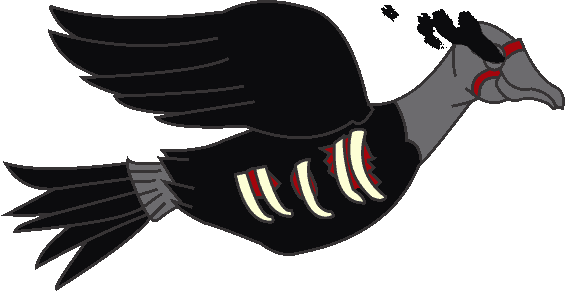
\includegraphics[height=0.2 \textheight]{Imagenes/zopilote}
	\caption{Concepto de diseño del Zopilote.}
	\label{fig:zopilote}
\end{figure}
\subsection{Encuentro:}
En el nivel 6 (ver apartado \ref{Nivel:Niv06}).
\subsection{Habilidades:}
\begin{itemize}
	\item Vuelo en picada (ver apartado \ref{hab.Vpicada}).
\end{itemize}
\subsection{Patrón de ataque:}
Su movimiento se da en dos puntos horizontales: A y B. Realiza un patrullaje de punto A al B y del B al A, cada vez que regresa a alguno de los puntos por segunda vez consecutiva ejecuta la habilidad de vuelo en picada (ver apartado \ref{hab.Vpicada}).
\subsection{Bloques de animación:}
\begin{itemize}
		\item Animación vuelo.
		\item Animación caída en picada.
	\end{itemize}
